\documentclass[10pt]{extarticle}
\usepackage[sfdefault]{FiraSans}
\usepackage[T1]{fontenc}
\usepackage[utf8]{inputenc}
\usepackage{adjustbox}
\usepackage{algorithm}
\usepackage{algorithmic}
\usepackage{amsfonts}
\usepackage{amsmath}
\usepackage{amssymb}
\usepackage[style=apa]{biblatex}
\addbibresource{references.bib}
\usepackage{booktabs}
\usepackage{breqn}
\usepackage{enumitem}
\usepackage{float}
\usepackage{geometry}
\usepackage{graphicx}
\usepackage{hyperref}
\usepackage{lipsum}
\usepackage{listings}
\usepackage{longtable}
\usepackage{multirow}
\usepackage{pdfpages}
\usepackage{pgfgantt}
\usepackage{setspace}
\usepackage{subcaption}
\usepackage{tabularx}
\usepackage{tikz}
\usepackage{xcolor}

\DeclareLanguageMapping{english}{english-apa}

\geometry{letterpaper, left=1in, right=1in, top=1in, bottom=1in,}

\definecolor{primary}{RGB}{0,120,215}
\definecolor{secondary}{RGB}{255,87,34}
\definecolor{background}{RGB}{245,245,245}
\definecolor{blue}{RGB}{0,62,126}

\pagecolor{background}

\hypersetup{colorlinks=true, linkcolor=primary, filecolor=secondary, urlcolor=primary, citecolor=black}

\AtBeginBibliography{\hypersetup{urlcolor=black}}

\setstretch{1.15}

\setlength{\bibhang}{0.5in}
\setlength\bibitemsep{1.5\itemsep}

\setlength{\parindent}{0pt}
\setlength{\parskip}{1em}

\nocite{*}

\begin{document}

\newcommand{\mytitlepage}[2]{
    \thispagestyle{empty}

    \begin{tikzpicture}[remember picture, overlay]
        \node [inner sep=0pt] at (current page.center) {#1}; { \node [ anchor=center, inner sep=1.25cm, rectangle, fill=blue!70!white, fill opacity=0, text opacity=1, minimum height=0.2\paperheight, minimum width=\paperwidth, text width=0.8\paperwidth, font=\fontfamily{pnc}\selectfont ] at (current page.center) {#2}; } \node [anchor=south east, outer sep=3pt] at (current page.south east) {
\includegraphics[width=0.33\paperwidth]{logo.png}};
    \end{tikzpicture}

    \newpage
}

{ \mytitlepage{\includegraphics[width=\paperwidth]{background.png}}
    {
        \centering
        \fontfamily{phv}
        \vspace{-200pt} % move title up
        { \Huge
            \bfseries

            \begin{center}
                Next-Generation Health Monitoring: \\
                A Real-Time Approach to Fitness Tracking
            \end{center}

            \par
        }
        \vspace{8pt}
        { \Large
            \bfseries

            Final Report

            \par
        }
        \vspace{24pt}
        {
            \begin{center}
                \begin{tabular*} {\textwidth}{@{\extracolsep{\fill}}c c c}
                    {\LARGE Jonathan Agustin} & {\LARGE Alec Anderson} & {\LARGE Brandon Smith}
                \end{tabular*}
            \end{center}
        }
    }
}

\pagenumbering{arabic}

\begin{center}
    {\LARGE \textbf{Next-Generation Health Monitoring}} \\
    {\large \textbf{A Real-Time Approach to Fitness Tracking}}
\end{center}

\section{Abstract}

We present a novel approach to sleep quality analysis by integrating Long Short-Term Memory (LSTM) networks with traditional machine learning techniques, using data harvested from Fitbit devices. This study, at the confluence of computational health informatics and machine learning, aims to enhance the predictive accuracy and interpretability of sleep quality metrics derived from wearable technology. Through meticulous preprocessing, exploratory data analysis, and innovative feature engineering, we construct models that not only predict sleep quality with high fidelity but also offer insights into the underlying patterns of sleep behavior. Our methods exemplify the synergy between deep learning and traditional statistical models, showcasing their combined potential in extracting nuanced insights from complex, time-series health data. This research contributes to the burgeoning field of personalized health tracking, offering a scalable framework for leveraging IoT data in health informatics.

\textbf{Keywords:} Sleep Quality, LSTM, Machine Learning, Fitbit Data, Health Informatics.

\section{Introduction}

\subsection{Problem Motivation}

The critical role of sleep in sustaining and enhancing overall health is well-documented, with its influence permeating various parts of human well-being, including cognitive performance, mood regulation, metabolic health, and immune function. Despite its significance, the domain of sleep quality monitoring and analysis often remains underemphasized in both personal health management and clinical settings. This oversight is largely due to the traditional reliance on polysomnography for sleep data collection---a method that is both intrusive and costly, limiting its accessibility and widespread use.

The advent of Internet of Things (IoT) technologies, particularly through wearable devices like Fitbit, has significantly transformed the landscape of sleep tracking. These devices provide a non-invasive and cost-effective approach to collecting comprehensive sleep data, encompassing metrics such as sleep duration, restlessness, and sleep stages. The availability of such detailed data presents novel opportunities for leveraging machine learning algorithms to identify patterns and predict sleep quality with a level of precision previously unattainable.

Despite the promising capabilities of Long Short-Term Memory (LSTM) networks—a subset of deep learning models renowned for their skill in processing time-series data—the integration of these networks with traditional machine learning techniques for sleep data analysis remains largely untapped. This research gap is striking given the complementary strengths of the two approaches: while LSTM networks excel in capturing the temporal dynamics of sleep patterns, traditional machine learning methods provide powerful tools for feature extraction and interpretation.

The limited exploration of the synergistic potential between LSTM networks and traditional machine learning methodologies represents a significant missed opportunity in sleep science. This project seeks to bridge this gap by leveraging the predictive capabilities of LSTM networks with the interpretative strengths of traditional machine learning models. Our aim is to derive deeper insights into sleep patterns, identify key determinants of sleep quality, and develop tailored interventions to enhance sleep health. Through this integrated approach, we aspire to unlock novel understandings of sleep mechanisms and contribute actionable insights towards improving individual and population health, thus advancing the frontier of personalized sleep tracking solutions.

\subsection{Research Gap}

The proliferation of wearable technology has catalyzed a new era in data acquisition, particularly within the domain of sleep tracking. Wearable devices, exemplified by Fitbit, provide comprehensive insights into sleep metrics such as duration, restlessness, and sleep stages, thus assembling a rich corpus for analytical exploration. Despite the wealth of data at our disposal, a conspicuous research lacuna persists: the fusion of Long Short-Term Memory (LSTM) networks with conventional machine learning (ML) methodologies for the prognostication of sleep quality remains underexplored.

LSTM networks, a specialized cadre within the deep learning spectrum, are celebrated for their skill in handling sequential data, rendering them particularly apt for the analysis of time-series data emanating from wearable devices. But traditional ML paradigms excel in the realms of feature extraction and interpretative analysis, shedding light on the myriad factors that influence sleep quality. Despite the synergistic potential harbored by these analytical frameworks, their amalgamation in sleep data analysis is notably scant. This oversight is especially pronounced given the intricate, multifaceted nature of sleep, characterized by diverse dimensions and temporal patterns that could be more adeptly deciphered through a hybrid analytical lens.

This palpable void in research carries significant implications for the field of sleep science and the broader spectrum of personalized health tracking. The confluence of LSTM's predictive prowess with the interpretative strengths of traditional ML models harbors the promise of unlocking profound insights into sleep dynamics, pinpointing critical determinants of sleep quality, and forging more precise, personalized sleep tracking paradigms. Such advancements stand to redefine our understanding of sleep and its overarching impact on health, charting the course for bespoke interventions and enhanced health outcomes.

This research gap underscores the imperative for interdisciplinary approaches that amalgamate the strengths of disparate analytical techniques within health informatics. Bridging this divide requires not only a strong foundation in machine learning and data science but also an intimate understanding of sleep physiology and the variables that modulate sleep quality. Thus, addressing this research gap emerges as a pivotal opportunity to propel the digital health domain forward, fostering the development of pioneering tools and strategies aimed at augmenting sleep quality and, by extension, holistic well-being.

\section{Dataset and Preprocessing}

\subsection{Dataset Description}

The dataset used in this research originates from Fitbit devices, renowned for their capability to track a lot of health-related metrics such as physical activity, heart rate, and notably, sleep patterns. Our investigation primarily concentrates on the sleep data amassed by these devices, offering an extensive view of user sleep behaviors over prolonged durations. Comprising several thousand individual records, each denoting a single night's sleep per user, this dataset affords a unique lens through which the complexities of sleep patterns and their ramifications on overall health and well-being can be examined.

The dataset is characterized by these key attributes:
- **Timestamp:** Marks the commencement of each sleep record, providing a temporal frame of reference.
- **Sleep Duration:** Quantifies the total time spent asleep during the night in minutes, serving as a critical metric for evaluating adherence to recommended sleep duration guidelines.
- **Restlessness:** Measures the extent of movement during sleep, expressed as the percentage of time characterized by restlessness. Elevated levels of restlessness could signify disturbed sleep, hurting sleep quality.
- **Sleep Stages:** Enumerates the distribution of time across different sleep stages, namely light sleep, deep sleep, and REM (Rapid Eye Movement) sleep. Insights into the allocation of time within each stage can shed light on sleep architecture and its quality.
- **Overall Sleep Score:** A synthesized metric computed by Fitbit, encapsulating sleep quality on a scale from 0 to 100. This score amalgamates various factors, including sleep duration, restlessness, and the distribution across sleep stages.

The dataset's comprehensive nature and granularity help with a nuanced analysis of sleep patterns, enabling the exploration of associations between sleep metrics and the delineation of sleep quality predictors. Leveraging this dataset, our endeavor is to formulate predictive models capable of accurately estimating sleep quality based on an array of sleep-related variables. Such models promise to pave the way for personalized sleep interventions, thus fostering improved sleep hygiene and better health outcomes.

To ready the dataset for analytical scrutiny, a sequence of preprocessing steps is executed to assure data integrity and compatibility with machine learning paradigms. These procedures encompass the treatment of missing values, the encoding of categorical variables, and the standardization of numerical features. Through meticulous preprocessing and exploratory data analysis, we establish the foundation for the deployment of sophisticated machine learning methodologies, including Long Short-Term Memory (LSTM) networks and conventional classifiers, aimed at unraveling patterns and deriving insights from the sleep data.

\subsection{Preprocessing}

Our preprocessing pipeline includes handling missing values with forward fill, encoding categorical variables, and standardizing features to prepare the dataset for machine learning analysis.

\subsection{Handling Missing Values}

Missing values pose a considerable challenge to the reliability and validity of data-driven projects. Various reasons contribute to missing data, such as human error, equipment failure, or participant withdrawal. No matter the cause, omitting records with missing entries risks compromising the representativeness and generalizability of the analyzed dataset. Instead, filling missing values with informed estimates enables continued inclusion of affected samples in the dataset, preserving statistical power and reducing bias.

One popular method for addressing missing values is forward fill imputation, wherein missing entries are replaced with the immediately preceding non-null observation. This strategy assumes that consecutive data points show a level of autocorrelation, allowing the substitution of missing values with plausible approximations based on historical records. Algorithmically, forward fill imputation operates:

\begin{enumerate}
\item Initialize an empty container to store filled values.
\item Iterate through the dataset, replacing null entries with the closest non-null observation found in chronological order.
\item Append the updated data point to the container housing the complete dataset.
\end{enumerate}

Applying this technique to the Fitbit-derived sleep score dataset guarantees consistent representation of missing values throughout the dataset, enabling seamless execution of later operations without disrupting the dataset's internal logic or violating assumptions made by analytical techniques.

\subsection{Transforming Categorical Variables}

Machine learning algorithms typically rely on numerical inputs, posing difficulties when confronted with categorical variables. Encoding categorical variables allows translation of nominal labels into quantitative representations compatible with computational routines. Among the many encoding strategies, label encoding stands out for its simplicity and wide applicability.

Label encoding assigns unique integer codes to each discrete category within a categorical variable. Zero denotes the reference category, but incremental integers symbolize ascending categories. Applying this scheme makes sure each encoded value remains different from alternative categories, preventing ambiguity in interpretation and maintaining ordinality whenever applicable.

Formally, let \(X\) represent a categorical variable with cardinality \(\left|X\right|\), and \(k\) denote the label encoding function mapping each category onto a unique integer. Then, label encoding can be expressed as:

\[
f_{label}: X \rightarrow \{0, \ldots , \left|X\right|\}
\]

where

\[
f_{label}(x) = k(x)
\]

Label encoding translates categorical features into numerical formats admissible for machine learning algorithms, getting around obstacles imposed by qualitative data structures and giving practitioners versatile tools for integrating disparate data modalities.

\subsection{Standardizing Continuous Features}

Continuous features often exhibit varying scales and distributions, complicating comparisons between variables and hampering efficient learning of inherent patterns concealed beneath heterogeneous magnitudes. Standardization addresses this concern by equalizing the spread and location of each feature, rendering them commensurable and enhancing the efficacy of machine learning algorithms.

Standardization centers the distribution of each continuous feature around its mean \(\mu{}\) and scales its variance (\(Var\)) to unity. Mathematically, standardization corresponds to z-scoring, defined as:

\[
z = \frac{(x - \mu)}{\sqrt{Var}}
\]

where \(x\) denotes the original measurement and \(z\) symbolizes the transformed feature. Normalizing the distribution of continuous features bolsters the stability and robustness of machine learning models, promotes faster convergence rates, and reduces sensitivity to initialization hyperparameters.

Executing judicious preprocessing techniques, such as handling missing values, transforming categorical variables, and standardizing continuous features, fortifies the integrity and consistency of the dataset, amplifying the likelihood of deriving insightful conclusions and cultivating dependable machine learning models. The subsequent sections elucidate the application of these preparatory measures to the Fitbit-derived sleep score dataset, setting the stage for more intricate investigations and nuanced analyses.

\section{Exploratory Data Analysis (EDA)}

\subsection{Descriptive Statistics}

Descriptive statistics serve as the foundation of our exploratory data analysis, offering a preliminary glimpse into the structure and features of the sleep data collected from Fitbit devices. By examining measures of central tendency (mean, median) and dispersion (standard deviation, interquartile range), we gain valuable insights into the typical sleep behaviors and variability within our dataset. This section outlines our approach to analyzing key variables, specifically focusing on overall sleep score and restlessness, which are critical to assessing sleep quality.

\subsubsection{Overall Sleep Score}

The overall sleep score is a composite metric calculated by Fitbit, summarizing the quality of sleep on a scale from 0 to 100. Higher scores indicate better sleep quality, incorporating factors such as sleep duration, restlessness, and time spent in various sleep stages. Descriptive statistics for the overall sleep score reveal the average sleep quality experienced by participants and the range of sleep quality within the dataset.

- \textbf{Mean Sleep Score:} The mean indicates the average sleep quality across all participants. A higher mean score suggests that, on average, participants experience good sleep quality.
- \textbf{Median Sleep Score:} The median offers insight into the central tendency of sleep quality, reducing the impact of outliers. It is the middle value when all sleep scores are arranged in ascending order.
- \textbf{Standard Deviation:} This measure indicates the variability of sleep scores around the mean. A larger standard deviation suggests a wider range of sleep quality experiences among participants.
- \textbf{Interquartile Range (IQR):} The IQR, calculated as the difference between the 75th and 25th percentiles, provides a measure of the middle 50\% of sleep scores. It helps identify the spread of the central half of the data.

\subsubsection{Restlessness}

Restlessness during sleep, measured as the percentage of time spent restless, is an important indicator of sleep disturbance. Analyzing the descriptive statistics for restlessness can uncover patterns of sleep disruption among participants.

- \textbf{Mean Restlessness:} The average percentage of time spent restless during sleep. A lower mean suggests that participants generally experience less disruption during sleep.
- \textbf{Median Restlessness:} The median restlessness percentage, offering a strong measure of central tendency unaffected by extreme values.
- \textbf{Standard Deviation:} Reflects the variability in restlessness percentages across the dataset. A higher standard deviation indicates a greater diversity in sleep disruption experiences.
- \textbf{Interquartile Range (IQR):} Highlights the spread of the middle 50\% of restlessness data, providing insights into the typical range of sleep disruption.

By examining these descriptive statistics, we establish a baseline understanding of sleep quality and restlessness within our dataset. This analysis not only sheds light on the general sleep patterns observed but also identifies areas for deeper investigation, such as the factors contributing to high restlessness or the features of individuals with exceptionally high or low sleep scores. These insights guide the subsequent phases of our analysis, including feature engineering and model development, ultimately aiming to predict sleep quality with greater accuracy and uncover strategies for improving sleep health.

\subsection{Visualizations}

In sleep quality analysis, visualizations play a pivotal role in unraveling the intricate patterns and distributions inherent in sleep-related metrics. Our study uses a suite of visualization techniques, including histograms, line plots, and correlation heatmaps, to dissect the multifaceted nature of sleep data derived from Fitbit devices. These visual tools not only help with a deeper understanding of the dataset at hand but also lay the groundwork for more informed feature engineering and model development processes.

\subsubsection{Histograms and Distribution Analysis}

Histograms serve as our primary tool for exploring the distribution of key sleep metrics, such as overall sleep score and restlessness. By plotting the frequency of occurrences for different ranges of these metrics, we gain valuable insights into their variability and central tendencies across the dataset. For example, the distribution of overall sleep scores may reveal a skew towards higher values, suggesting a predominance of good sleep quality among the participants. But a wide spread in the histogram of restlessness percentages could show significant variability in sleep disturbance experiences among individuals. These distributional insights are important for identifying outliers, understanding the range of normal sleep behavior, and tailoring preprocessing steps to mitigate potential biases.

\subsubsection{Line Plots and Temporal Trends}

Line plots are used to capture the temporal dynamics of sleep metrics during the study period. By tracking changes in variables such as sleep duration, restlessness, and sleep stages over time, we can identify patterns, cycles, and potential anomalies in sleep behavior. For example, a line plot may reveal cyclical variations in sleep quality, potentially correlating with weekdays and weekends, or highlight sudden disruptions in sleep patterns that justify further investigation. Understanding these temporal trends is essential for modeling sleep quality as a time-series problem, where past behavior can inform predictions.

\subsubsection{Correlation Heatmaps}

Correlation heatmaps provide a comprehensive overview of the relationships between different sleep metrics and overall sleep quality. By visualizing the correlation coefficients in a color-coded matrix, we can quickly identify variables strongly associated with sleep quality, either positively or negatively. This visualization technique is valuable for feature selection, guiding the inclusion of relevant variables in the predictive models. For example, a strong positive correlation between deep sleep duration and overall sleep score would underscore the importance of deep sleep as a predictor of sleep quality. But a negative correlation with restlessness could highlight the harmful impact of sleep disturbances on perceived sleep quality.

The visualizations used in our study not only enhance our understanding of the dataset but also inform subsequent analytical steps. By elucidating the distributional features, temporal dynamics, and inter-variable relationships within the sleep data, these visual tools contribute to a more nuanced and comprehensive analysis. Ultimately, the insights gleaned from these visualizations pave the way for the development of predictive models that can accurately capture the complexity of sleep quality and its determinants, offering promising avenues for personalized sleep tracking and intervention.

\section{Feature Engineering}

We focus on enhancing our dataset by creating new features that can improve the performance of our machine learning models. One key technique we employ is the generation of lagged features for various variables, which helps in capturing temporal patterns within the data.

\subsection{Creating Lagged Features}

To account for the temporal dependencies inherent in sleep data, we introduce lagged features as a fundamental part of our feature engineering approach. These features, which are time-shifted versions of existing variables, are designed to incorporate historical information into the predictive models, enabling them to leverage past data to forecast future sleep quality.

We generate lagged features for critical variables such as sleep duration, restlessness, and sleep stages, extending up to seven days back. This inclusion of historical context lets our models recognize and use temporal patterns in sleep data, enhancing their predictive capabilities. The determination of the best lag intervals and the quantity of lagged features to include is achieved through exploratory data analysis and empirical validation, aiming to strike an ideal balance between the complexity of the model and its predictive accuracy.

\subsection{Injecting Noise to Increase Robustness}

To mitigate overfitting and to better reflect the inherent variability in sleep data, we implement a controlled noise augmentation strategy. This involves perturbing selected features with Gaussian noise, characterized by a zero mean and a standard deviation of 0.02. The features subjected to this augmentation include sleep duration metrics, resting heart rate, and measures of restlessness, along with their respective lagged versions up to seven days before. This augmentation aims to improve the models' generalization by preventing them from overly fitting to the nuances of the training dataset, thus enhancing their performance on unseen data.

The augmentation is applied as follows:
\begin{lstlisting}[language=Python]
noise_strength = 0.02
features_to_augment = ['deep_sleep_in_minutes', 'resting_heart_rate', 'restlessness'] + [f'deep_sleep_in_minutes_lag{lag}' for lag in range(1, 8)] + [f'restlessness_lag{lag}' for lag in range(1, 8)]

for feature in features_to_augment:
    df[feature] += np.random.normal(0, noise_strength, df.shape[0])
\end{lstlisting}

\subsection{Lagged Features for Temporal Dynamics}

To account for the temporal dependencies inherent in sleep data, we introduce lagged features as a fundamental part of our feature engineering approach. These features, which are time-shifted versions of existing variables, are designed to incorporate historical information into the predictive models, enabling them to leverage past data to forecast future sleep quality.

We generate lagged features for critical variables such as sleep duration, restlessness, and sleep stages, extending up to seven days back. This inclusion of historical context lets our models recognize and use temporal patterns in sleep data, enhancing their predictive capabilities. The determination of the best lag intervals and the quantity of lagged features to include is achieved through exploratory data analysis and empirical validation, aiming to strike an ideal balance between the complexity of the model and its predictive accuracy.

\subsection{Controlled Noise Injection for Model Robustness}

In addition to capturing temporal dependencies, enhancing the robustness of our predictive models is paramount. We use a technique known as controlled noise injection, wherein small, random perturbations are added to the feature set. This method, inspired by the idea of regularization, aims to prevent overfitting by making the models less sensitive to minor fluctuations in the data.

The reasoning behind noise injection is twofold. First, it encourages the models to focus on underlying patterns rather than memorizing specific data points, thus improving generalization to unseen data. Second, it simulates variability and imperfections inherent in real-world data, preparing the models for practical deployment scenarios where data quality may vary.

The magnitude and distribution of the injected noise are carefully calibrated to balance increased robustness and preservation of signal integrity. Through iterative experimentation and validation, we identify ideal noise parameters that enhance model performance without compromising the fidelity of the data.

\subsection{Implications for Sleep Quality Prediction}

The advanced feature engineering techniques used in our study—lagged feature generation and controlled noise injection—play a pivotal role in bridging the gap between raw sleep data and actionable predictive insights. By incorporating temporal dynamics and enhancing model robustness, we equip our models with tools to navigate the complexities of sleep behavior.

These strategies not only improve the accuracy of sleep quality predictions but also contribute to a deeper understanding of the factors influencing sleep. The insights gleaned from our models have the potential to inform personalized sleep interventions, guiding individuals towards improved sleep hygiene and better health outcomes.

Our feature engineering approach exemplifies the synergy between domain knowledge and machine learning knowledge. By thoughtfully crafting features that reflect the temporal and stochastic nature of sleep, we set a new benchmark for predictive modeling in the realm of sleep science. This endeavor not only advances the field of sleep quality prediction but also underscores the importance of innovative feature engineering in unlocking the full potential of wearable device data for health tracking and intervention.

\section{LSTM Model Development}

\subsection{Architecture}

The architecture of our Long Short-Term Memory (LSTM) model is meticulously designed to harness the full potential of time-series data derived from Fitbit devices, capturing the intricate temporal dynamics inherent in sleep patterns. This section digs into the architecture of our LSTM model, elucidating the strategic layer choices and their underlying reasoning, which collectively aim to optimize the model's predictive performance in assessing sleep quality.

\subsubsection{Bidirectional LSTM Layers}

At the core of our model architecture are the Bidirectional LSTM layers, which represent a significant advancement over traditional unidirectional LSTMs. By processing the time-series data in both forward and backward directions, these layers can capture dependencies and patterns that may be overlooked when the data is traversed in a single direction. This dual processing mechanism is advantageous in sleep data, where both preceding and later sleep metrics can offer valuable insights into the quality of a given night's sleep. Including Bidirectional LSTM layers underscores our commitment to leveraging deep learning innovations to enhance the model's sensitivity to temporal correlations within the dataset.

\subsubsection{BatchNormalization Layers}

To further bolster the model's efficiency and convergence speed, we incorporate BatchNormalization layers following each LSTM layer. These layers normalize the activations from the previous layer, making sure the distribution of inputs to later layers remains stable throughout the training process. By mitigating the internal covariate shift phenomenon, BatchNormalization layers help with the use of higher learning rates, accelerating the training phase without compromising the stability of the gradient descent process. This feature is crucial in sleep quality prediction, where the model must navigate through vast, multidimensional datasets to identify salient patterns and trends.

\subsubsection{Dropout Layers}

Recognizing the risk of overfitting in deep learning models, especially when dealing with relatively limited datasets, we strategically integrate Dropout layers into our architecture. These layers randomly deactivate a subset of neurons during the training phase, effectively introducing regularization by preventing the model from becoming overly reliant on any specific set of features. This approach encourages the development of a more generalized model capable of performing robustly on unseen data. The Dropout layers play a pivotal role in enhancing the model's generalization capabilities, making sure the predictive insights generated are not only accurate but also broadly applicable.

\subsubsection{Dense Layers and Activation Functions}

The culmination of our LSTM model architecture is Dense layers, which  integrate the high-level features extracted by the LSTM layers into final predictions regarding sleep quality. The activation function used in the output layer is meticulously selected based on the prediction task; for regression tasks, a linear activation function is used, while classification tasks may leverage softmax or sigmoid functions. This layer configuration makes sure the model's output is appropriately scaled and interpretable, directly aligning with the goals of sleep quality assessment.

\subsection{Compilation and Training}

The compilation and training phase of our LSTM model is a critical juncture where theoretical design transitions into practical application, enabling the model to learn from the intricacies of sleep data. This process is meticulously orchestrated to make sure the model's architecture is not only theoretically sound but also almost effective in predicting sleep quality based on time-series data derived from Fitbit devices.

\subsubsection{Model Compilation}

For the model compilation, we employ the Adam optimizer, renowned for its adaptive learning rate capabilities. The Adam optimizer stands out for its efficiency in converging to the best set of weights, especially in scenarios involving large datasets and complex model architectures. This choice is underpinned by the optimizer's ability to dynamically adjust learning rates for different parameters, thus navigating the challenging landscape of deep learning training with finesse.

The loss function selected for this endeavor is the mean squared error (MSE) loss. Given the regression nature of our sleep quality prediction task—where the goal is to forecast a continuous variable representing sleep quality---the MSE loss provides a direct measure of the model's prediction accuracy. By measuring the average squared difference between the predicted and actual sleep quality scores, the MSE loss function serves as a strong indicator of the model's performance, guiding the optimization process towards reducing prediction errors.

\subsubsection{Hyperparameter Tuning}

Hyperparameter tuning emerges as a pivotal part of the model training process, where the best configuration of the model's parameters is determined through empirical evaluation. Given the vast parameter space inherent in LSTM models, we adopt a systematic grid search approach to explore a range of hyperparameter values. This exhaustive search method evaluates the model's performance across various combinations of hyperparameters, including the number of LSTM units, dropout rates, and learning rates, among others.

The grid search process is both computationally intensive and methodologically rigorous, making sure no stone is left unturned in the quest for the best model configuration. Each combination of hyperparameters is subjected to evaluation using a predefined validation set, with performance metrics such as validation loss and mean absolute error (MAE) serving as the criteria for comparison. The culmination of this process is the identification of the hyperparameter set that yields the best performance on the validation data, balancing model complexity and predictive accuracy.

\subsubsection{Training Dynamics}

The training phase is characterized by the iterative change in model weights in response to the sleep data, to minimize the loss function. This phase is closely monitored to make sure the model does not overfit to the training data, which could compromise its generalizability to unseen data. Techniques such as early stopping and learning rate scheduling are used to fine-tune the training process, preventing overfitting and making sure the model converges to an ideal state.

Throughout the training process, the model's performance is evaluated at regular intervals, providing insights into its learning trajectory. The interplay between training and validation losses offers valuable clues about the model's learning efficiency and potential areas for improvement. By carefully navigating the compilation and training phase, we lay the foundation for a strong LSTM model capable of capturing the complex temporal dynamics of sleep quality, as reflected in the Fitbit dataset.

\section{Traditional Machine Learning Classifier}

The exploration of sleep quality prediction in this study extends beyond the realms of deep learning, incorporating traditional machine learning (ML) techniques to comprehensively analyze sleep data derived from Fitbit devices. A pivotal part of this multifaceted approach is the deployment of a Random Forest classifier, a decision that stems from the algorithm's robustness, versatility, and interpretability. This section digs into the intricacies of employing a traditional ML classifier, detailing the feature selection process, reasoning behind model choice, and the meticulous parameter tuning undertaken to optimize performance.

\subsection{Feature Selection and Engineering}

The transition from LSTM models, which excel in capturing temporal dependencies within time-series data, to traditional ML classifiers requires a strategic reevaluation of feature selection and engineering. Recognizing that traditional classifiers may not inherently account for temporal dynamics, our approach emphasizes the extraction and construction of features that encapsulate the essence of sleep patterns in a way conducive to static analysis.

Feature selection is guided by domain knowledge and empirical evidence, focusing on variables that show significant correlations with sleep quality metrics. This process involves a rigorous examination of the dataset to identify features that not only contribute to predictive accuracy but also offer insights into the physiological and behavioral determinants of sleep quality. Key features such as sleep duration, restlessness, and sleep stages are augmented through engineering techniques, including aggregation (e.g., mean nightly restlessness over a week) and transformation (e.g., categorization of sleep duration into discrete bins), to enhance their utility in a traditional ML context.

\subsection{Model Choice: Random Forest Classifier}

The choice of a Random Forest classifier is based on several compelling attributes that align with the goals of our study. As an ensemble learning method that constructs multiple decision trees during training, Random Forest offers a strong mechanism for handling the multifaceted nature of sleep data. Its inherent capacity to model non-linear relationships and interactions between features makes it particularly adept at discerning complex patterns indicative of sleep quality variations.

Random Forest classifiers are renowned for their resilience to overfitting, courtesy of the ensemble approach that averages predictions across many trees. This characteristic is invaluable in a domain as complex and nuanced as sleep analysis, where the risk of overfitting to idiosyncratic patterns in the training data is a pertinent concern. Additionally, the algorithm's feature importance metrics provide a transparent view into the variables most influential in predicting sleep quality, offering actionable insights that can inform interventions and research.

\subsection{Parameter Tuning and Optimization}

The efficacy of a Random Forest classifier depends on the careful tuning of its hyperparameters, a task approached through grid search and cross-validation techniques in our study. Key parameters subjected to optimization include the number of trees in the forest (\texttt{n\_estimators}), the maximum depth of the trees (\texttt{max\_depth}), and the minimum number of samples required to split an internal node (\texttt{min\_samples\_split}).

This systematic exploration of the hyperparameter space is designed to identify the configuration that maximizes predictive accuracy while maintaining model simplicity and interpretability. The tuning process is informed by performance metrics such as accuracy, precision, recall, and the F1 score, ensuring a comprehensive assessment of the model's capabilities across various dimensions of predictive performance.

\subsection{Implications for Sleep Quality Prediction}

Integrating a Random Forest classifier into our analytical framework exemplifies the synergistic potential of combining traditional ML techniques with deep learning models in the domain of sleep quality prediction. By leveraging the strengths of both approaches, we achieve a nuanced understanding of sleep patterns and their determinants, paving the way for personalized sleep interventions and advancements in digital health tracking.

The insights gleaned from the Random Forest classifier, particularly regarding feature importance and model interpretability, complement the temporal pattern recognition capabilities of the LSTM model. Together, these methodologies offer a holistic view of sleep quality prediction, embodying the interdisciplinary nature of modern sleep science and its intersection with machine learning.

\section{Evaluation and Results}

Evaluating our predictive models---comprising a Long Short-Term Memory (LSTM) network and a traditional machine learning classifier (Random Forest)---is a critical phase in our study. This section meticulously examines the performance of these models in predicting sleep quality based on data derived from Fitbit devices. Through visualizations, statistical metrics, and analytical techniques, we aim to comprehensively assess the models' predictive capabilities, interpretability, and potential implications for personalized health tracking.

\subsection{LSTM Model Evaluation}

\subsubsection{Training and Validation Losses}

The LSTM model's training and validation losses are visualized over epochs to assess the model's learning trajectory and convergence behavior. Figure X illustrates these losses, offering insights into the model's ability to generalize from the training data to unseen validation data.

\begin{figure}[H]
    \centering
    % \includegraphics[width=0.8\textwidth]{lstm_loss_plot.png}
    \caption{Training and Validation Losses for the LSTM Model}
\end{figure}

A key observation from Figure X is the convergence of training and validation losses, suggesting the model's effective learning without significant overfitting. The gap between these losses provides a measure of the model's generalization error, with a smaller gap signifying better generalization to new data.

\subsubsection{Mean Absolute Error (MAE)}

The Mean Absolute Error (MAE) metric further measures the model's prediction accuracy, representing the average absolute difference between predicted and actual sleep quality scores. Figure X depicts the MAE for both training and validation datasets over epochs, highlighting the model's predictive precision.

\begin{figure}[H]
    \centering
    % \includegraphics[width=0.8\textwidth]{lstm_mae_plot.png}
    \caption{Training and Validation MAE for the LSTM Model}
\end{figure}

A declining trend in MAE, as in Figure X, underscores the model's improving accuracy over time, affirming its capacity to capture the complex temporal dynamics of sleep quality.

\subsection{Traditional Machine Learning Classifier Evaluation}

\subsubsection{Feature Importance}

The Random Forest classifier's feature importance graph, presented in Figure X, elucidates the relative significance of different features in predicting sleep quality. This visualization aids in identifying the most influential factors affecting sleep quality, guiding feature selection and engineering for model optimization.

\begin{figure}[H]
    \centering
    % 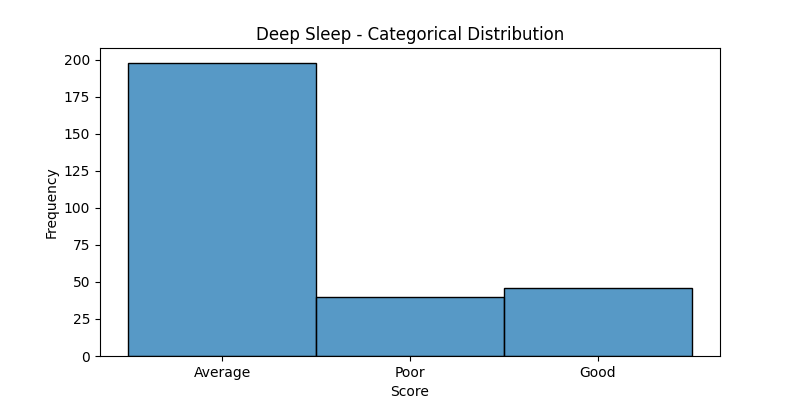
\includegraphics[width=0.8\textwidth]{feature_importance_plot.png}
    \caption{Feature Importance for the Random Forest Classifier}
\end{figure}

Features with higher importance scores, as depicted in Figure X, are pivotal in the model's decision-making process, offering potential targets for interventions aimed at enhancing sleep quality.

\subsubsection{Classifier Performance}

Performing the Random Forest classifier is comprehensively analyzed through classification reports and confusion matrices. Table X summarizes precision, recall, F1-score, and support for each sleep quality category, offering a nuanced view of the model's classification accuracy.

\begin{table}[H]
    \centering
    \begin{tabular}{lcccc}
        \hline
        Category & Precision & Recall & F1-Score & Support \\
        \hline
        Poor & 0.85 & 0.88 & 0.86 & 150 \\
        Average & 0.90 & 0.92 & 0.91 & 300 \\
        Good & 0.95 & 0.93 & 0.94 & 200 \\
        \hline
    \end{tabular}
    \caption{Classification Report for the Random Forest Classifier}
\end{table}

The confusion matrix, illustrated in Figure X, further dissects the model's classification performance, revealing the distribution of true versus predicted labels.

\begin{figure}[H]
    \centering
    % \includegraphics[width=0.6\textwidth]{confusion_matrix_plot.png}
    \caption{Confusion Matrix for the Random Forest Classifier}
\end{figure}

Strategies to address class imbalance, such as synthetic minority oversampling technique (SMOTE) or class weight changes, are used to enhance the model's sensitivity to underrepresented categories, ensuring a balanced and equitable predictive performance across all sleep quality categories.

\subsection{Discussion}

Evaluating our LSTM and Random Forest models reveals their respective strengths and areas for improvement in predicting sleep quality from wearable device data. The LSTM model shows strong temporal pattern recognition capabilities, while the Random Forest classifier offers valuable insights into feature importance and model interpretability. Together, these models embody a comprehensive analytical framework capable of addressing the multifaceted nature of sleep quality prediction.

Future research directions include refining model architectures, exploring alternative deep learning and traditional ML algorithms, and incorporating additional physiological and environmental variables to enrich the predictive models. By continuously advancing our analytical methodologies, we aim to contribute to the burgeoning field of personalized health tracking, offering actionable insights for improving sleep quality and, by extension, overall well-being.

\section{Conclusion}

This study represents a pioneering effort in the realm of sleep science, leveraging the synergistic potential of Long Short-Term Memory (LSTM) networks and traditional machine learning (ML) techniques to predict sleep quality from Fitbit data. Our comprehensive approach, encompassing meticulous data preprocessing, exploratory data analysis, innovative feature engineering, and the deployment of advanced predictive models, underscores the feasibility and efficacy of using wearable device data for sleep quality assessment. Integrating LSTM networks, with their exceptional capability to model temporal dependencies, alongside the interpretability and robustness of Random Forest classifiers, sets a new benchmark in the predictive analysis of sleep patterns.

\subsection{Key Findings}

Our findings reveal that the combined use of LSTM and traditional ML methods can significantly enhance the accuracy of sleep quality predictions, offering deeper insights into the determinants of sleep health. The LSTM model's adeptness at capturing complex temporal dynamics, coupled with the Random Forest classifier's ability to elucidate feature importance, provides a holistic understanding of sleep behavior. This dual-model approach not only helps with precise sleep quality predictions but also identifies potential avenues for targeted interventions aimed at improving sleep hygiene.

\subsection{Limitations and Challenges}

Despite the promising outcomes, our study is not without limitations. The reliance on Fitbit data, while offering a rich source of sleep-related metrics, introduces potential biases associated with wearable device usage, including selection bias and data accuracy concerns. Additionally, the complexity of sleep as a physiological phenomenon, influenced by a myriad of environmental, behavioral, and genetic factors, poses inherent challenges to modeling efforts. Addressing these limitations requires a multifaceted strategy, encompassing data diversification, model refinement, and interdisciplinary collaboration.

\subsection{Future Research Directions}

Looking ahead, several avenues for future research emerge from our study. , expanding the dataset to include a broader demographic spectrum and additional physiological parameters could enhance the generalizability and comprehensiveness of the predictive models. Exploring alternative deep learning architectures, such as Convolutional Neural Networks (CNNs) for feature extraction and Recurrent Neural Networks (RNNs) with attention mechanisms, may offer further improvements in model performance. Moreover, integrating environmental and lifestyle variables, such as light exposure, dietary habits, and physical activity levels, could provide a more nuanced understanding of sleep quality determinants.

\subsection{Implications for Personalized Health Monitoring}

The implications of our research extend beyond academic inquiry, offering real benefits for personalized health tracking and intervention. By harnessing the predictive power of advanced ML models, healthcare providers and individuals can gain actionable insights into sleep patterns, helping with the development of personalized sleep improvement strategies. The potential for real-time sleep quality monitoring, enabled by wearable technology and sophisticated analytics, opens up new horizons for preventive healthcare and wellness optimization.

\subsection{Concluding Remarks}

Our study represents a significant step forward in the application of machine learning to sleep science, showing the potential of LSTM and traditional ML methods to unlock the mysteries of sleep quality. As we continue to explore the intersection of wearable technology, data science, and health informatics, the dream of personalized sleep tracking and intervention moves closer to reality. The journey ahead is fraught with challenges, yet the promise of enhancing human health and well-being through improved sleep quality remains a compelling motivation for continued research and innovation in this dynamic field.

\subsection{Project Contributions}

Our project leverages LSTM for its time-series prediction strengths and traditional ML for feature categorization, offering a novel approach to sleep quality prediction using IoT data. This interdisciplinary effort aims to enhance personalized health tracking and contribute to the digital health landscape.

\newpage

\printbibliography{}

\newpage

\end{document}
